% --------------------------------------------------------------------------
% Report template for BIR projects
% Report template with support for Portuguese and English languages
% Change language {brazil or english} in \documentclass as per the examples
% This template has support for the ABNT citing format
%
% Original version: jan/2019
% https://github.com/
%
% Based on ABNTEX2 and the thesis template
% --------------------------------------------------------------------------
\documentclass[
%\DeclareUnicodeCharacter{200B}{}
% --------------------------------------------------------------------------
% classe memoir . options
12pt,					% tamanho da fonte
openright,				% cap. começam em pág ímpar (ins pág vazia caso preciso)
twoside,				% para impressão em verso e anverso. Oposto a oneside
a4paper,				% tamanho do papel
% --------------------------------------------------------------------------
% classe abntex2 . options
%chapter=TITLE,			% títulos de capítulos convertidos em letras maiúsc.
%section=TITLE,			% títulos de seções convertidos em letras maiúsc.
%subsection=TITLE,		% títulos de subseções convertidos em letras maiúsc.
%subsubsection=TITLE,	% títulos de subsubseções convertidos em letras maiúsc.
% --------------------------------------------------------------------------
% Opções de IDIOMA do pacote babel
english,
brazil
]{ABNT/abntex2_report}
% --------------------------------------------------------------------------
% Pacotes básicos
\usepackage{lmodern}			% Usa a fonte Latin Modern
\usepackage[T1]{fontenc}		% Selecao de codigos de fonte.
\usepackage[utf8]{inputenc}		% Codificacao do documento (conversão automática dos acentos)
\usepackage{indentfirst}		% Indenta o primeiro parágrafo de cada seção.
\usepackage{color}				% Controle das cores
\usepackage{graphicx}			% Inclusão de gráficos
\usepackage{microtype} 			% para melhorias de justificação
\usepackage{lipsum}
\usepackage[brazilian,hyperpageref]{backref} % páginas com citações na bibliog.
%\usepackage[alf,abnt-etal-list=0,abnt-etal-cite=3,abnt-emphasize=bf]{abntex2cite}
\usepackage[alf]{abntex2cite}
%
\usepackage{lastpage}			% Usado pela Ficha catalográfica
%\usepackage{subfig}
\usepackage{supertabular}       % tabela na capa do documento
\usepackage{booktabs}
\usepackage[table,xcdraw]{xcolor}
\usepackage{adjustbox}
\usepackage{amssymb,amsmath,mathrsfs}
\usepackage{algorithm,algpseudocode}
\usepackage{pgfplots}
\usepackage{tikz}
\usepackage{titlesec}
\usepackage{ragged2e}
\usepackage{tocloft}
\usepackage{threeparttable}
\usepackage{etoolbox}
\usepackage[normalem]{ulem}
\usepackage{yaacro}
\usepackage[none]{verlab}
%\usepackage{fontspec}
%\setmainfont{Helvetica Light}
\usepackage{lscape}
%\usepackage[graphicx]{realboxes}
\usepackage{rotating}
\usepackage{wrapfig}
\usepackage{caption}
\usepackage{subcaption}
\usepackage{dirtytalk}
\usepackage{pdfpages}
\usepackage{threeparttable}
\usepackage{hyperref}
%\hypersetup{draft}
\usepackage{float}
\DeclareUnicodeCharacter{200B}{}
% --------------------------------------------------------------------------%
% Configurações do PDF final
\definecolor{blue}{RGB}{41,5,195}
\makeatletter
\hypersetup{
	%pagebackref=true,
	pdftitle={\@title},
	pdfauthor={\@author},
	pdfsubject={\@title},
	%pdfsubject={\imprimirpreambulo},
	pdfcreator={LaTeX with abnTeX2},
	pdfkeywords={abnt}{latex}{abntex}{abntex2}{\imprimirpalavraschave},
	colorlinks=true,       		% false: boxed links; true: colored links
	linkcolor=blue,          	% color of internal links
	citecolor=blue,        		% color of links to bibliography
	filecolor=magenta,      	% color of file links
	urlcolor=blue,
	bookmarksdepth=4
}
%\makeatother
% --------------------------------------------------------------------------
% Posiciona figuras e tabelas no topo da página quando adicionadas sozinhas
% em um página em branco. Ver https://github.com/abntex/abntex2/issues/170
%\makeatletter
\setlength{\@fptop}{5pt} % Set distance from top of page to first float
\makeatother
% --------------------------------------------------------------------------
% Formatação
\newcommand\tab[1][1cm]{\hspace*{#1}}
\apptocmd{\thebibliography}{\justifying}{}{}
\renewcommand{\ABNTEXsectionfont}{\bfseries}
\titlespacing*{\chapter}{0pt}{0pt}{12pt}
\titlespacing*{\section}{0pt}{6pt}{6pt}
\titlespacing*{\subsection}{0pt}{6pt}{6pt}
\titlespacing*{\subsubsection}{0pt}{6pt}{6pt}
% --------------------------------------------------------------------------
% Rearranja os finais de cada estrutura
\algrenewtext{EndWhile}{\algorithmicend\ \algorithmicwhile}
\algrenewtext{EndFor}{\algorithmicend\ \algorithmicfor}
\algrenewtext{EndIf}{\algorithmicend\ \algorithmicif}
\algrenewtext{EndFunction}{\algorithmicend\ \algorithmicfunction}
% --------------------------------------------------------------------------
% Espaçamentos entre linhas e parágrafos
\setlength{\parindent}{1.3cm} % linha
\setlength{\parskip}{0.2cm} % parágrafo, tente também \onelineskip
% --------------------------------------------------------------------------
% Informações de dados para CAPA e FOLHA DE ROSTO
\prodtecnica{001 / 2020}
\titulo{Aplicações Práticas da SunBurn}
\tiporelatorio{Final}
\nomeprojeto{Sistemas Produtivos}
\outrossubtitulos{~} % opcional
\autores{
	Jéssica Lima Motta\\
	Leonardo Mendes de Souza Lima\\
	Vinícius José Gomes de Araujo Felismino\\
	Pedro Paulo Ventura Tecchio\
}
% \newcommand{\autoresexternos}{
% 	John Marston\\
% 	Frank West\
% }
\local{Salvador\\Bahia, Brasil}
\data{Setembro de 2020}
% \classificacao{( ) Confidencial  (X) Restrito  ( )  Uso Interno  ( ) Público}
% \revisao{01}
% \tabelacutter{000}
% \palavraschave{1. Manipulator. 2. Simulation. 3. Computer vision.}
% \classificacaoassunto{000} % sNúmero de Classificação do assunto
%\parceirologo{logos/x.png}
%------------------------------------------------------------------
% Finalização das configurações da capa
%
%
%------------------------------------------------------------------
% Acrônimos :: Chamar no texto como \ac{DoF}
\begin{acgroupdef}[list=acronyms]
	\acdef{CEP}{Controle Estatístico de Processos}
	\acdef{MRP}{Manufacturing Resource Planning}
	%
	%
	%
\end{acgroupdef}
% --------------------------------------------------------------------------
% Criação do sumário
\makeindex
%
\begin{document}
	% \frenchspacing
	\imprimircapa
	% \imprimircatalografica
% --------------------------------------------------------------------------
% Sumário executivo
	% \ABNTEXchapterfont\large\textbf{\execsummarytitlename}
	% \begin{flushleft}
	% 	\normalsize
	% 	\justify
	% 	\normalfont
	% 	O projeto de Manipuladores - Desafio.2, também conhecido como \textbf{xxxxx} se configura sob o Programa de Formação de Novos Talentos do Serviço Nacional de Aprendizagem Industrial, Departamento Regional da Bahia - Senai/DR/BA, sendo este o principal fomentador do programa.

	% 	O projeto foi considerado como início técnico do projeto o dia 00 de bolsoneiro de 2020.

	% 	O prazo de execução planejado é de xx meses.
	% \end{flushleft}
	% \clearpage
%------------------------------------------------------------------
% Resumo e abstract
	\ABNTEXchapterfont\large\textbf{\resumoatitlename}
	\begin{flushleft}
		\normalsize
		\justify
		\normalfont
		%resumo aqui
		%
		%
		%
	\end{flushleft}
	% \vspace*{1cm}
	% \newpage
	% %
	% \ABNTEXchapterfont\large\textbf{\resumobtitlename}
	% \begin{flushleft}
	% 	\normalsize
	% 	\justify
	% 	\normalfont
	% 	%abstract aqui
	% 	%
	% 	%
	% 	%
	% \end{flushleft}
	% \clearpage
% --------------------------------------------------------------------------
% Lista de figuras
	% \begin{flushleft}
	% 	\ABNTEXchapterfont\Large\textbf{\MakeUppercase\listadefigurasname}
	% \end{flushleft}
	% \vspace*{-36pt}
	% \pdfbookmark[0]{\listfigurename}{lof}
	% \normalsize
	% \listoffigures*
	% \cleardoublepage
% --------------------------------------------------------------------------
% Lista de tabelas
	% \begin{flushleft}
	% 	\ABNTEXchapterfont\Large\textbf{\MakeUppercase\listadetabelasname}
	% \end{flushleft}
	% \vspace*{-36pt}
	% \pdfbookmark[0]{\listtablename}{lot}
	% \normalsize
	% \listoftables*
	% \cleardoublepage
% --------------------------------------------------------------------------
% Lista de símbolos e abreviaturas
	% \begin{flushleft}
	% \ABNTEXchapterfont\Large\textbf{\MakeUppercase\listadesimbolsabrevtitlename}
	% 	\noindent
	% 	\vspace*{-06pt}
	% 	\pdfbookmark[0]{\listadesiglasname}{lot}
	% 	\normalsize
	% 	\normalfont
	% 	\aclist[list=acronyms]
	% \end{flushleft}
	% \newpage
% --------------------------------------------------------------------------
% Tabela de conteúdo
	% \begin{flushleft}
	% 	\ABNTEXchapterfont\Large\textbf{\MakeUppercase\glosariotitlename}
	% \end{flushleft}
	% %\pagebreak
	% \vspace*{-36pt}
	% \pdfbookmark[0]{\contentsname}{toc}
	% \normalsize
	% \normalfont
	% \tableofcontents*
	% \justify
% --------------------------------------------------------------------------
% Formatação, remover espaço depois dos títulos
	\setlength\beforechapskip{-24pt}
	\setlength\afterchapskip{12pt}
	\textual
	\pagestyle{plain}
	\normalsize
	\justify
	\normalfont
% --------------------------------------------------------------------------
% Conteúdo do relatório
	\chapter{INTRODUÇÃO}
\label{chap:intro}
Como parte da etapa de desenvolvimento do projeto de Automação de Operações com \textit{\acs{ROV}}, \cite{pybullet}

\cite{sivvcev2018underwater}

Entretanto

%------------------------------------------------------------------
\section{Objetivos}
\label{sec:obj}
Projetar e construir uma prova de conceito para subsidiar a análise de viabilidade técnica-econômica de automatizar operações submarinas com manipuladores de \textit{\acs{ROV}}, também conhecido como veículo submarino operado remotamente.


%------------------------------------------------------------------
\section{Justificativa} %motivação
\label{sec:just}
Nesta etapa da automação de um manipulador, 


%------------------------------------------------------------------
\section{Organização do relatório}
\label{sec:org}
Este documento está organizado da seguinte forma, o capítulo 

%----------------------- marcado
\section{Resumo da empresa}
\label{sec:rese}
A SunBurn é uma empresa de nome fictício que atua no desenvolvimento, implantação e operação de projetos de energia renovável. No Brasil, é sediada no sul do país e opera nas regiões Norte, Sul e Nordeste.

Os projetos da empresa, nos Ambientes de Contratação Regulada (ACR) e Contratação Livre (ACL), somam 642 Megawatts de potência vendida. Todos os empreendimentos são monitorados à distância por meio do Centro de Operações localizado na sede da SunBurn, na região Sul.
A SunBurn estabelece um modelo de negócios com maior segurança e rentabilidade a seus investidores, mantendo o compromisso de fornecer energia limpa e confiável.

Os empreendimentos têm como característica fundamental a qualidade, apresentando altos fatores de capacidade e geração garantida. Aliado ao modelo de gestão da SunBurn, que segue os princípios do ESG (Environmental, Social and Corporate Governance), a alta tecnologia e profissionais qualificados garantem confiabilidade na operação.

A sustentabilidade é fator indissociável da estratégia de negócios da SunBurn. Nas regiões onde a empresa atua, as operações têm foco na redução de impactos ambientais, no desenvolvimento das comunidades da região e na segurança dos colaboradores.





	\include{sections/02gestaodasoperaçoes}
	\include{sections/03medidasdedesempenhodaoperaçao}
	\chapter{A estratégia de produção}
\label{chap:estrategia_da_producao}
%Neste capítulo será explicado como formular a estratégia de produção de uma empresa industrial visando atender o seu objetivo geral de desempenho. Uma estratégia de produção consiste em converter as intenções contidas em ações práticas como projetos concretos, planos e melhorias. Para isso, será explicado como a matriz "importância x desempenho" pode auxiliar na definição de estratégias de produção.

A estratégia de produção analisa o processo global da função de produção da empresa industrial como um todo. Por isso, caso exista, ela se preocupa com as outras partes da corporação, com as unidades de negócio (marketing, finanças, recursos humanos entre outras) e com o local onde o negócio esta inserido (concorrentes, clientes externos etc). Além disso, tem o objetivo de manter a área de operações adaptadas às mudanças externas como fatores ambientais dentre outros. Logo, a operação terá maiores chances de enfrentar os problemas futuros. Com isso, é mais garantido que as organizações possam ter níveis sustentáveis de vantagens competitivas \cite{correa2000administracao}.

Ainda segundo o autor, a matriz \textit{importância $\times$ desempenho}, mostrada na Figura \ref{fig:matriz_importancia_desempenho}, é uma ferramenta que deve ser utilizada para a priorização dos objetivos da função de operações. Essa matriz, possui duas dimensões: uma delas refere-se à importância relativa dada pelos clientes aos critérios de desempenho, utilizando a escala de nove pontos e a outra envolve uma classificação, também com uma escala de nove pontos, do desempenho de cada objetivo contra os níveis de desempenho atingidos pelos concorrentes.

\begin{figure}[H]
  \caption{Matriz importância $\times$ desempenho}
  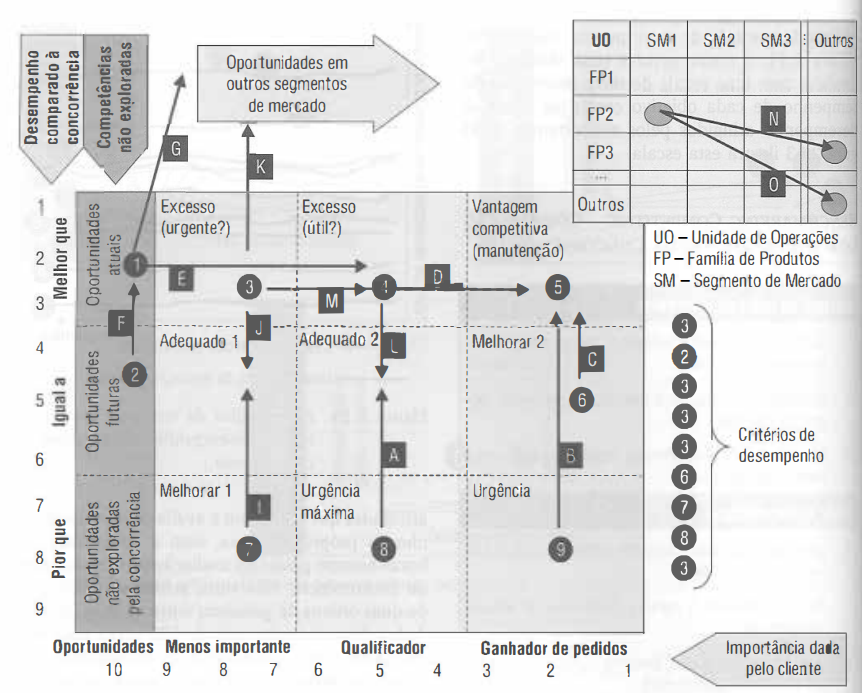
\includegraphics[width =1\textwidth]{images/impor_desem.png}
  \label{fig:matriz_importancia_desempenho}
  \caption*{Fonte: \cite{correa2000administracao}}
\end{figure}

O cruzamento das duas dimensões (importância dos critérios para o mercado e desempenho nos critérios comparado à concorrência) permite identificar regiões específicas na matriz, conforme mostrado na Figura \ref{fig:matriz_importancia_desempenho}. Esta traz uma arranjo eficaz no que se refere a estabelecerem prioridades e a partir disso, designar os esforços e recursos de melhoria estratégica em operações. Vale salientar que para se obter esta matriz é necessário ter em vista a análise de um dado conjunto homogêneo de clientes (conhecido por ``segmento de mercado'') que compra um conjunto homogêneo de produtos (conhecido por ``família de produtos'') \cite{correa2000administracao}.



\section{Aplicação Prática}
\label{sec:estrategia_da_producao_aplicacao}
	\chapter{Tipos de processos de produção industrial} 
\label{chap:tipos_de_processo_de_producao} 

\section{Sec1} 
\label{sec:tipos_de_processo_de_producao_sec1} 


\section{Aplicação Prática} 
\label{sec:tipos_de_processo_de_producao_aplicacao}
	\chapter{O projeto do produto}
\label{chap:projeto_do_produto}

Existem diversos tipos de projetos necessários à implementação e funcionamento de uma empresa industrial. O presente capítulo foca no projeto do produto, que é uma atividade complexa e subdividida em diversas etapas: geração do conceito, triagem do conceito, projeto preliminar, avaliação do projeto preliminar, construção de protótipos e projeto final do produto.  O projeto final do produto tem como resultados entregáveis o conceito final, o pacote de documentos e a descrição de processos. O fluxograma mostrado na Figura \ref{fig:projeto_produto} apresenta, em linhas gerais, as etapas presentes neste processo, mesmo que, na prática os projetistas avancem ou retrocedam pelas etapas de forma iterativa. Serão descritas a seguir cada etapa deste processo na ordem em que geralmente ocorrem.

\begin{figure}[H]
  \centering
  \caption{Fluxograma das etapas do projeto do produto.}
  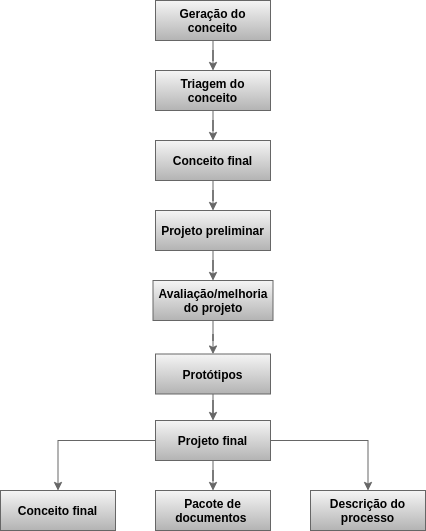
\includegraphics[width=.7\textwidth]{images/projeto_produto.png}
  \caption*{Fonte: Adaptado \cite{slack2006administracao} }
  \label{fig:projeto_produto}
\end{figure}

%! aqui esta sendo feita uma itemização diferente da feita no capítulo anterior
\textbf{Geração do conceito:} É a primeira etapa para o desenvolvimento do projeto de um produto. É nesta fase que se elabora um resumo completo do conjunto de benefícios que o produto, quando fabricado, deverá proporcionar ao seu usuário, podendo este ser ou não cliente direto da empresa. Tais benefícios devem corresponder às necessidades, desejos e expectativa do usuário, portanto, esta é uma atividade sob responsabilidade da equipe de \textit{marketing}, pois são eles que fazem a ponte entre o usuário e a equipe operacional da empresa.

\textbf{Triagem do conceito:} Nesta etapa ocorre uma avaliação entre as diversas alternativas de conceitos concebidas na etapa anterior. Esta avaliação, segundo \cite{slack2006administracao}, deve considerar a importância de cada solução proposta, de modo que possam ser feitas escolhas entre elas. Cada opção é avaliada a partir de três categorias de critérios: a viabilidade - ``Quão difícil é o projeto?'', a aceitabilidade - ``O projeto vale a pena?'' e a vulnerabilidade - ``O que pode dar errado?''.

\textbf{Conceito final:} Concluídas as avaliações da etapa anterior, obtém-se um conceito final do produto, que servirá de base para toda a parte de detalhamento técnico: forma, design, materiais, funcionalidades, resistência, segurança, durabilidade em uso e disponibilidade após a vida útil do produto. É importante lembrar que nesta etapa, ainda, não é apresentado os detalhes técnicos do produto, mas é indispensável para o referido detalhamento.

\textbf{Projeto preliminar:} Nesta etapa se inicia o detalhamento das informações de natureza técnica, fundamentais para a concepção do produto. Os documentos gerados nesta fase são, a princípio, os mesmos que farão parte da documentação final do projeto.

\textbf{Avaliação/melhoria do projeto:} O projeto do produto é uma atividade interativa, ou seja, está sujeita a sucessivas otimizações a medida em que evolui. Existem diversas técnicas ou ferramentas para a revisão e melhoria do projeto de um produto, dentre elas, destacam-se: o \ac{QFD}, engenharia de valor e os testes acelerados de resistência.

\textbf{Protótipos:} Antes da empresa colocar seu produto em produção regular, ela constrói exemplares iniciais do seu produto. O objetivo desta etapa é realizar testes e ensaios para observar o desempenho do protótipo em relação aos conceitos e projetos em fase de avaliações e melhorias.

\textbf{Projeto final:} A última etapa do processo consiste em elaborar um documento que contenha o conjunto de informações e especificações técnicas, que não deixem margem à dúvidas ou equívocos, para a produção do produto para o mercado. Segundo \cite{slack2006administracao}, a documentação final do projeto de um produto deve conter: o conceito final definitivo, ``pacote de documentos do produto'' (estrutura do produto, lista de materiais, especificações técnicas e seus componentes) e a descrição do processo de fabricação/montagem do produto (fluxograma).


\section{Aplicação Prática}
\label{sec:projeto_do_produto_aplicacao}

De certa forma, uma vez que o produto da SunBurn é energia elétrica, que deve ser entregue de forma estabelecida pelas instruções normativas da \ac{ANEEL} e de acordo com as características adotadas pelas linhas de transmissão aonde a unidade produtiva será instalada, o projeto de produto se dá apenas na adequação das características de tensão, forma de onda e frequência da energia produzida. Assim, o conceito final do produto pode ser caracterizado como energia elétrica com certo nível de tensão na faixa de kV e onda senoidal com frequência de 60 Hz.

A descrição do processo de fabricação deste produto foi realizada no Capítulo \ref{chap:tipos_de_processo_de_producao}, haja visto que o mesmo é fábricado de forma contínua. Em linhas gerais, a energia solar é transformada em energia elétrica com corrente contínua e baixa tensão pelos painéis fotovoltaicos. Em seguida a mesma é convertida para energia elétrica com corrente alternada pelos inversores, com subsequente elevação das tensões nos transformadores para o nível das linhas de transmissão.

Não foi possível o acesso ao pacote de documentos do processo de fabricação da SunBurn.	
	\chapter{Projetos de novas instalações produtivas (localização, capacidade e rede de operações)} 
\label{chap:projetos_de_novas} 

\section{Cadeia de suprimentos: estrutura, verticalização e terceirização} 
\label{sec:projetos_de_novas_supply_chain} 
A cadeia de suprimentos de um processo produtivo é a relação da empresa com seus fornecedores e clientes, e a relação destes com seus fornecedores e clientes como descrita na Figura \ref{fig:supply_chain}. Nesta figura é possível perceber que os fornecedores que lidam diretamente com a operação são os de primeira camada, e os fornecedores dos fornecedores compõem a segunda camada, e estes fazem parte da montante do processo. Igualmente para o lado jusante, que tem os clientes de primeira camada, contato direto com a operação, e clientes dos clientes, que são os de segunda camada.
\par Além disso nota-se que fornecedores e clientes de primeira camada fazem parte da rede imediata de fornecimento, e a rede completa é chamada de rede total de suprimentos.


\begin{figure}[H]
    \centering
    \caption{Cadeia de Suprimentos (supply chain)}
    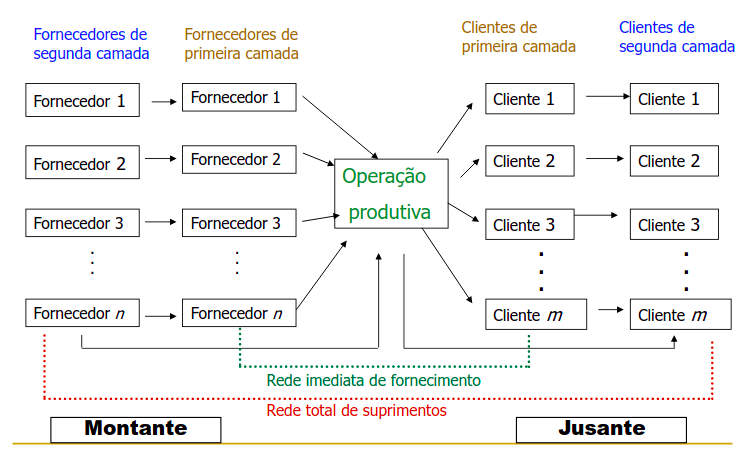
\includegraphics[scale=0.65]{images/supply_chain.png}
    \caption*{Fonte: \cite{supplychain}}
    \label{fig:supply_chain}
\end{figure}
  
\par A importância de entender toda a rede é vital para a competitividade da empresa devido aos seguintes aspectos: identificar a relações imediatas, isso ajuda a conhecer melhor fornecedores e clientes; identificar elos significativos, saber quais partes da rede contribuem para alcançar os objetivos de desempenho valorizados pelos clientes finais, esta análise começa primeiramente pela parte da jusante e depois pela montante da rede a partir dos quais mais contribuem para o serviço do consumidor final, e por último, focar em questões de longo prazo, alguns elos dessa rede podem gerar situações como greves ou parada de máquina que ocasione uma interrupção no fluxo da operação, é importante estudar a possibilidade de ajudar ou substituir esse elo mais fraco.



\section{Aplicação Prática} 
\label{sec:projetos_de_novas_aplicacao}
Para a SunBurn a escolha da localização onde seus parques de energia solar seriam implantados foi escolhida conforme os dois fatores fundamentais para esse tipo de sistema produtivo: um grande espaço e estudo prévio durante dois anos para verificar o índice de irradiação solar naquele local. 
\par Por esses motivos a reunião Nordeste foi escolhida para implementar os parques solares, já que esta dispõe dos dois elementos fundamentais.

\par A cadeia de suprimentos da SunBurn encontra-se descrita na Figura \ref{fig:cadeia_suprimentos_sunburn}. Nesta figura encontram-se definidas as relações da montante (fornecedores) e da jusante (cliente) com a operação produtiva. Também são identificados os fornecedores fixos e os sob cotação e demanda, além dos fluxos de serviço e de informação que existe entre cada elemento deste fluxograma. 


\begin{figure}[H]
    \centering
    \caption{Cadeia de Suprimentos da SunBurn.}
    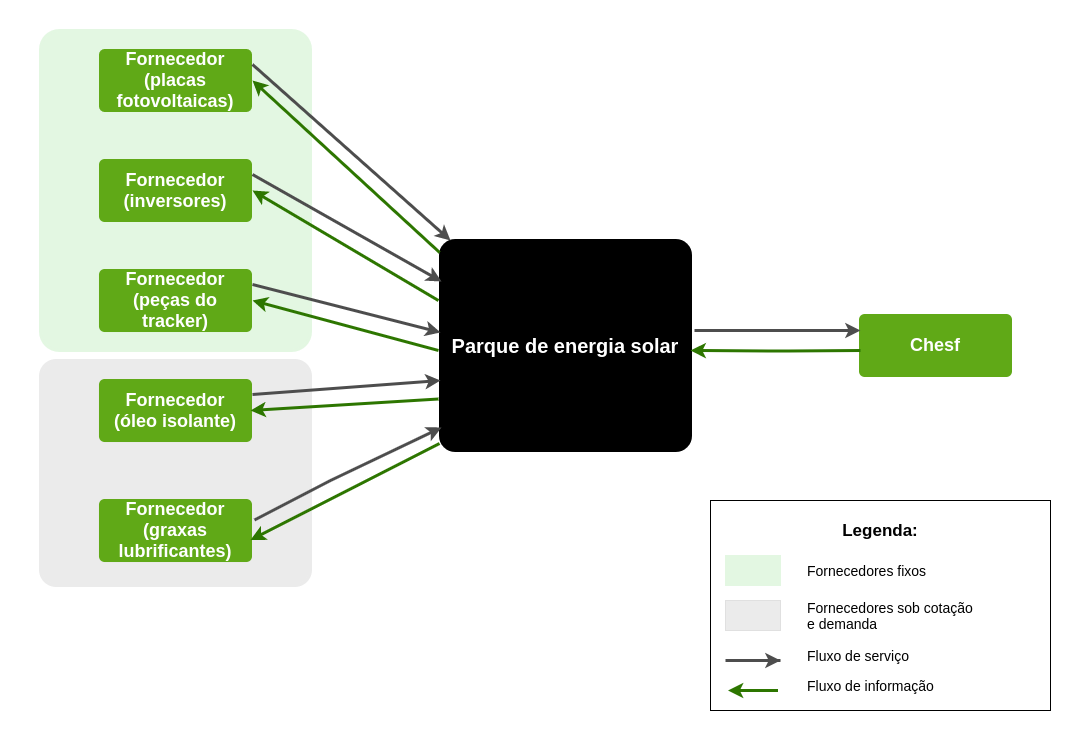
\includegraphics[width=1\textwidth]{images/cadeia_suprimentos_sunburn.png}
    \caption*{Fonte: Autoria própria.}
    \label{fig:cadeia_suprimentos_sunburn}
\end{figure}
  


	\chapter{O projeto do arranjo físico ("Lay-out")} 
\label{chap:projeto_do_arranjo} 
Arranjo físico ou lay-out dos equipamentos, é a disposição que os equipamentos possuem na fábrica, de modo que proporcionem a máxima eficiência dentro do processo produtivo.

OS principais tipos de arranjos físicos são o Posicional ou fixo, arranjo em que os equipamentos e operadores movem-se durante as operações; Físico por Processo, onde os equipamentos possuem posicionamento fixo; Físico Celular ou Células de Produção, onde os materiais fluem somente através de suas células específicas e o arranjo Físico por Produto (em linha), onde os materiais fluem através de equipamentos fixos, por um único e exclusivo roteiro, do início ao fim do processamento.

Antes de escolher o lay-out é importante que se considere todo o fluxo do processo da produção. Cada tipo de processo produtivo se encaixa em um dos quatro modelos mais comuns de arranjos físicos. Quantidade do produto a ser produzido, variedade de produtos que serão produzidos e o tipo de produto a ser produzido são os principais fatores a serem considerados antes da escolha do lay-out de produção.

Compreender o fluxo de trabalho da fábrica, o tipo de elemento a ser produzido, suas especificações  e volume são fatores determinantes na escolha do lay-out de produção. É também primordial posicionar os postos de trabalho próximos as máquinas para economizar tempo de percurso, mesmo mantendo o espaço reservado às áreas de segurança.
 


\section{Sec1} 
\label{sec:projeto_do_arranjo_sec1} 
 
\section{Aplicação Prática} 
\label{sec:projeto_do_arranjo_aplicacao}
	\chapter{Tecnologia - Recurso essencial para a competitividade da empresa industrial} 
\label{chap:tecnologia_recurso} 

\section{Tecnologia do Produto X Tecnologia do Processo} 
\label{sec:tecnologia_prod_process} 
  Tecnologia é o estudo sistemático sobre técnicas, processos, métodos e instrumentos de domínio da atividades humana. No setor industrial, este ofício representa o controle destas técnicas e também a capacidade de implementação de novas funcionalidades em máquinas para que estas possam operar de forma autônoma e sem o conhecimento do seu funcionamento interno. Em resumo, a tecnologia pode ser descrita como a arte de desenvolver e utilizar novas ferramentas.

  É definida como Tecnologia do produto aquela introduzida no produto e foi usada na criação do seu projeto ou no decorrer do seu desenvolvimento. De acordo com o Manual de Apoio ao Preenchimento da Pintec (2014), a inovação de produto consiste em criar modificações nos atributos dos bens ou serviços, tais como mudanças operacionais e na forma como ele é percebido pelos consumidores.

  A tecnologia empregada na rotina de produção de um produto, destinada a fazer com que sejam atingidas as metas estabelecidas pela empresa é chamada Tecnologia de Processo. O tipo de produto a ser produzido é quem dita a tecnologia usada no processo industrial, ao lado da quantidade e volume que serão fabricados.

  É exemplo de tecnologia de processos a empregada na produção de materiais. O uso de robôs e outras máquinas vem crescendo e se consolidando como algo indispensável. O uso de máquinas de corte, furadeiras e CNC complementam a tendencia no uso da automação. 

  O processamento de informações, assim como a TI, vem avançando e se popularizando exponencialmente. Tem a intenção de ser abrangente e atua como técnologia principal ou auxiliar em quase todos os ramos de trabalho. 
  
  O emprego das tecnologias permitem a constante inovação de produtos e processos e garantem a presença competitiva no mercado. Produtos novos, modificados e mais eficientes aumentam a procura e melhoram a opinião do cliente a respeito da empresa.



 
 

\section{Aplicação Prática} 
\label{sec:tecnologia_recurso_aplicacao}
	\chapter{Introdução ao planejamento e controle da produção}
\label{chap:introducao_ao_planejamento}

Nesta seção mostram-se algumas definições e conceitos introdutórios sobre o \ac{PCP}, em especial, os métodos qualitativos e quantitativos de previsão de demanda a curto, médio e longo prazo. Para isso, primeiramente é necessário entender e distinguir os tipos de demandas existentes no mercado que serão vistos na seção a seguir.

\section{Tipos de demanda}
\label{sec:introducao_ao_planejamento_sec1}

O trabalho do \ac{PCP} tem como objetivo compatibilizar a capacidade de produção da empresa com a demanda a ser entendida, consequentemente, a demanda é quem dita a natureza do atendimento. Existem dois tipos básico de demanda: a independente e a dependente e suas características serão descritas a seguir.

\subsection{Demanda independente}

Este é o tipo mais frenquentemente utilizado pela grande maioria das empresas. De fato, este tipo de demanda ocorre quando as empresas fazem previsões sobre as quantidades de produtos/serviços que seus usuários comprarão em um período de tempo próximo, portanto, preparam-se para aquele atendimento na esperança de que a demanda será bem próxima da previsão. A demanda independente é comum em lojas de varejo, empresas prestadores de serviços pessoais e grande parte das indústrias de bens de consumo final.

\subsection{Demanda dependente}

A demanda dependente só ocorre em situações particulares e menos frequentes. Este tipo de demanda surge quando as empresas possuem, de antemão, as informações de que necessita para elaborar seus planos de produção de curto prazo, ou seja, ela não se atenta em fazer previsões ou estimativas sobre as quantidades de produtos/serviços que seus clientes adquirirão em um curto período de tempo. Essa demanda surge quando as empresas têm o conhecimento prévio da intenção do cliente, está associada a um um evento certo e quando há pedidos confirmados.

\section{Métodos de previsão de demanda}
%! todo Não sei se ta certo

Existem dois métodos para tratar as informações disponíveis das previsões de curto, médio e longo prazo que são as abordagens quantitativas e as abordagens qualitativas. Vale salientar que qualquer processo de previsão, no geral, vai conter tanto considerações de natureza mais qualitativa como considerações mais quantitativas a respeito dos dados disponíveis. As características destas duas técnicas serão descritas a seguir

\subsection{Método qualitativo}

Esse método é subjetivo pois reúne os fatores de julgamento e intuição das análises dos dados disponíveis. Estes fatores são úteis quando se espera que esses dados, mais subjetivos, possam ter a capacidade de explicar o futuro, ou quando os dados quantitativos precisos e completos são muito caros ou difíceis de serem obtidos. Existem 5 métodos qualitativos para a precisão de demanda:

\textbf{Método Delphi:} É um processo interativo que permite aos especialistas, mesmo distantes uns dos outros, reunir seus palpites ao processo de previsão. O objetivo deste processo é evitar que uma ou poucas opiniões predominem por fatores exógenos ao propósito de gerar boas previsões.

\textbf{Júri de Executivos:} Método em que se captura a opinião de pequenos grupos, em geral, de executivos de nível alto sobre alguma variável que se pretenda prever.

\textbf{Força de vendas:} Tal método consiste em unir as estimativas localizadas e desagregadas emitidas por cada vendedor, ou representante de força de vendas, e com isso será formado uma estimativa global.

\textbf{Pesquisa de mercado:} Esse método consiste em solicitar diretamente dos possíveis clientes ou consumidores sua intenção de compra futura.

\textbf{Analogia histórica:} Método que procura identificar produtos similares dos quais possuem dados para, por analogia, melhor estimar. %? estimar o que a demanada?

\subsection{Método quantitativo}

Esse método de previsão de demanda é baseado na análise das séries de dados históricos em que se busca identificar os padrões de comportamento, para que estes sejam então projetados para o futuro. Ou seja, a previsão do futuro é baseado em dados do passado.

\section{Aplicação Prática}
\label{sec:introducao_ao_planejamento_aplicacao}
A estrutura do parque permite fornecer até 60 MW, estipulado por contrato com a Chesf. A demanda é dependente por contrato firmado entre o cliente e a SunBurn. Contudo, a demanda de energia elétrica oscila durante o dia a dia, assim, deve-ser ter uma regulação prevista de acordo com dados históricos para a operação diária, caracterizando-se como o método quantitativo.

	\chapter{Planejamento agregado da produção} 
\label{chap:planejamento_agregado} 

Existem dois grupos de métodos, qualitativos e quantitativos, que são aplicados na previsão de demanda de curto, médio e longo prazo.
Planejamento e controle possuem uma forte correlação já que previsões podem conter muitas incertezas e controle ajuda a ajustar o plano.
O tempo aplicado para dimensionar curto, médio e longo prazo, depende de cada modelo de negócio. Por exemplo: hidrelétricas, longo prazo seriam décadas e no mundo da moda seriam no máximo um ano.

Para a unidade industrial tem-se a convenção:

\textbf{Longo prazo:} inclui-se futuros investimentos em novas instalações ou ampliações existentes.

\textbf{Médio prazo:} são as decisões tomadas ao longo de um ano.

\textbf{Curto prazo:} refere-se as atividades realizadas no dia a dia.

O planejamento agregado leva a resultados mais precisos do que ao realizar-se planejamento de forma detalhada.

Há duas formas de ajustar a capacidade à demanda de produção:

\textbf{Produção nivelada:} a empresa atende a demanda oscilante mantendo a produção constante ao longo do tempo. Dessa forma, independente das oscilações da demanda o nível da produção irá se manter constante, logo a produção estará ''nivelada''. 

\textbf{Produção acompanhada a demanda:} o ajuste da capacidade é realizado por meio do acompanhamento da demanda de forma a flexibilizar a capacidade produtiva conforme as variações da demanda.


\section{Aplicação Prática} 
\label{sec:planejamento_agregado_aplicacao}

A SunBurn utiliza o método de produção nivelada pois independente das oscilações da demanda mantém-se a produção constante de energia elétrica. Há algumas alterações na produção, conforme o dia, devido a irradiação solar ocorrida.

	\chapter{O CONTROLE DOS ESTOQUES}
\label{chap:controle_estoques}

Segundo \cite{slack2006administracao} o estoque é definido como todo e qualquer tipo de material acumulado na entrada de qualquer estágio do processo global de produção, ou de distribuição de produtos. Este acúmulo ocorre tanto quando o ritmo de processamento dos insumos for mais lento que o do estágio anterior como quando este ritmo for mais rápido, pois haverá esperas decorrentes das faltas momentâneas de materiais no estágio em questão.

Estoques entre quaisquer estágios do processo de produção e distribuição seriam indesejáveis e indicariam uma certa anomalia no processo, no que se refere à sincronia entre suas etapas. A seguir serão descritos alguns motivos pelos quais as empresas industriais optam por formar estoques.

\textbf{Incertezas da demanda:} Para o ambiente de demanda independente (incerta), as empresas fazem suas previsões de vendas e produz os produtos para atender essas previsões. Porém, tais previsões são frequentemente passíveis de incertezas, isto é, ora a demanda está acima da demanda real, ora abaixo. Para a primeira situação o resultado é a formação de estoques desnecessários, já para a segunda há falta de produtos para o cliente. Como, para todo negócio, a falta de produtos para o cliente deve ser evitada, a empresa deverá produzir além da previsão e consequentemente aumentará ainda mais a formação de estoques desnecessários, especialmente nas situações em que as previsões já estavam acima da demanda real.

\textbf{Incertezas da capacidade:} Esse motivo é baseado na possibilidade de ocorrer imprevistos como falhas dos equipamentos, das máquinas, falta de operadores e atrasos na entrega de matérias primas por parte dos fornecedores, que resultará na falta de produtos para o cliente. Por isso, as empresas costumam se prevenir contra todas estas incertezas através da formação de estoques de ``proteção''.

\textbf{Limitações impostas pelo próprio processo produtivo:} Alguns processos produtivos operam obrigatoriamente em determinadas quantidades mínimas, não sendo viável ou conveniente produzir-se em quantidades menores. Justamente por esta limitação que o processo produtivo, em alguns casos, poderá formar estoques, pois torna-se difícil conciliar a taxa de produção com a taxa de demanda do produto.

\textbf{Gargalos no processo produtivo:} Em algumas instalações industriais, é comum a existência de equipamentos do processo que têm uso universal, ou seja, por eles passam muitos dos modelos do mix de produtos. Estes equipamentos são os gargalos do processo produtivo e, consequentemente, causadores da formação de estoques intermediários de produtos em processamento. 

\textbf{Opção pela produção nivelada:} Quando as empresas optam por atender a sua demanda por intermédio de produção a nível constante, remanejando estoques, as quantidades excedentes de produtos produzidos nos períodos de baixa demanda servem para complementar a produção dos períodos de alta demanda. Esta decisão resulta na formação de estoques antecipados.

\textbf{Estoques no canal de distribuição:} O próprio canal de distribuição de um produto de consumo é um grande estoque de produtos em trânsito, que deve estar sempre preenchido, para que não falte produto para o cliente.


O cálculo destes estoques de segurança, do ponto de vista conceitual, basta adicionar uma quantidade suplementar ao lote de ressuprimento, quantidade esta suficiente para compensar os eventuais aumentos da demanda e/ou atrasos das entregas do material. Na área da produção, observa-se que alguns gerentes terminam por exagerar no dimensionamento do estoque de segurança, por não dispor de informações adequadas para o seu cálculo. Para auxiliar no dimensionamento adequado destas quantidades suplementares existem dois métodos frequentemente utilizados: O Lote Econômico de Compras (LEC) e a classificação ABC para os estoques.

%------------------------------------------------------------------
\section{Aplicação Prática}
\label{sec:controle_estoques_aplicacao}
No SAP ocorre o controle do insumo utilizado. Toda vez que um insumo é consumido é necessário dar baixa no sistema. E cada um dos insumos possui um limite mínimo diferente e quando chega-se a esse valor é disparado pelo sistema uma ordem de compra. 

//todo como é feito o controle de estoques da empresa?
	\chapter{O \textit{Manufacturing Resource Planning}}
\label{chap:manufacturing_resource_planning}

Com base no \ac{PAP}, visto anteriormente, e nas análises de gerenciamento de estoques, pode-se utilizar a ferramenta \ac{MRP} para programar as atividades diárias da produção. Esta ferramenta permite o planejamento e controle, a curto prazo, dos meios de produção quando existe uma demanda dependente que consiste na definição das quantidades e momentos para a realização da compra dos insumos, bem como, na colocação das ordens de produção.

No âmbito do planejamento e controle dos meios de produção sob demanda dependente, o \textit{software} \ac{MRP} auxilia na execução das aquisições dos materiais diversificados e em diferentes quantidades dos diversos fornecedores, no planejamento da disponibilidade dos equipamentos necessários para cada etapa do processamento do pedido e na conciliação das duas atividades anteriores de forma que os produtos demandados possam ser produzidos de acordo com as datas estipuladas no contrato com o cliente. Além disso, esta ferramenta também atua de forma a otimizar o processamento do pedido de forma que o processo como um todo ocorra de forma contínua e eficiente.

Destaca-se que o \ac{MRP} utiliza o conceito de programação para trás, isto é, as tarefas necessárias para o atendimento do pedido são programadas de trás para a frente iniciando na data de entrega do pedido para o cliente. Deste modo, não há previsão de folgas para eventuais atrasos, contudo os estoques podem ser minimizados e os pagamentos para os fornecedores ocorrem no mais tardar possível. Para o correto funcionamento do \ac{MRP}, o mesmo necessita conhecer o Plano Mestre, isto é, o detalhamento de todos os pedidos firmados entre a empresa e seus clientes, a composição do produto com detalhamento técnico e, finalmente, os prazos de entrega dos fornecedores e os níveis de estoque da empresa.


%------------------------------------------------------------------
\section{Aplicação Prática}
\label{sec:manufacturing_resource_planning_aplicacao}
A SunBurn utiliza a metodologia \ac{SAP} para realizar as aquisições dos seus insumos, conforme visto no Capítulo \ref{chap:controle_estoques}. Acredita-se que a mesma esteja correlacionada aos processos realizados pela ferramenta \ac{MRP}.

	\chapter{O fornecimento \textit{Just In Time}}
\label{chap:fornecimento_just_in_time}

Enquanto o \ac{MRP} pode ser entendido como uma ferramenta utilizada no gerenciamento do processo produtivo, o fornecimento \ac{JIT} constitui uma nova filosofia de trabalho em contraponto com as práticas adotadas nas empresas industriais até o seu surgimento. Esta filosofia é definida por possuir as seguintes intenções: o produto deve ser fornecido ao cliente (interno ou externo) instantaneamente na quantidade estritamente especificada e esperada, evitar quaisquer tipo de ``desperdício'' de recursos produtivos, realizar as atividades de forma compartilhada em grupo com envolvimento efetivo das pessoas envolvidas no processo produtivo, bem como, a promoção continuada do aprimoramento das atividades executadas.

Com o intuito de atingir os objetivos prescritos de forma economicamente viável, mantendo a sua competitividade, os seguintes elementos devem ser observados:

\textbf{Baixos investimentos:} emprego criativo de pequenas máquinas e equipamentos universais, ou seja, que podem ser utilizadas na produção de diversos produtos.

\textbf{Flexibilidade:} por utilizar máquinas universais, o sistema produtivo \ac{JIT} apresenta naturalmente maior flexibilidade no conjunto de produtos possíveis de serem fabricados.

\textbf{Baixos custos de produção:} talvez o aspecto mais relevante nesta filosofia, mas certamente o que a faz ser tão competitiva com os modelos tradicionais de produção, é a redução dos custos de produção. Os baixos custos são provenientes das práticas adotadas de redução de desperdício, sendo que o conceito adotado de desperdício igual a toda e qualquer atividade que não agrega valor ao produto. Assim, atividades como transporte de mercadorias, geração e armazenamento de estoques, bem como movimentação de pessoas de forma desnecessária são classificadas como desperdícios. Além destes, a produção de defeitos, falhas e deficiências nos produtos ou processos também se enquadram nesse conceito.

\textbf{Fluxo contínuo:} de produtos e processos, sem interrupções, suave e rápido.

\textbf{Melhoria permanente:} a ideologia e mentalidade de que os produtos e processos podem ser constantemente aprimorados dever ser criada e mantida em todas as pessoas envolvidas no processo produtivos.

%------------------------------------------------------------------
\section{Aplicação Prática}
\label{sec:fonercimento_just_in_time_aplicacao}
Não é, não trabalha conforme a demanda. Só é cobrado da SunBurn caso tenha irradiação solar e não esteja gerando energia elétrica.

//todo A SunBurn apresenta o sistema Just in time? Se sim, quais foram as dificuldades de implementação? Se não, quais seriam as dificuldades para implementar (temos que pensar)? 
	\chapter{O controle estatístico de processos}
\label{chap:controle_estatistico_de_processos}
No controle estatístico de processos são utilizadas ferramentas que auxiliam na interpretação dos dados coletados, para identificar a relação entre os defeitos e as causas ou auxiliar no desenvolvimento das atividades a serem desempenhadas.  Na seção \ref{sec:controle_estatistico_sec1} serão abordadas essas ferramentas e na seção \ref{sec:controle_estatistico_aplicacao} serão demonstradas quais dessas ferramentas são utilizadas pela SunBurn.

%------------------------------------------------------------------

\section{Ferramentas}
\label{sec:controle_estatistico_sec1}

\subsection{Diagrama de Correlação}
É utilizado de forma a verificar a relação dos problemas/defeitos encontrados com relação ao tempo (correlação temporal) ou relação entre problemas e suas possíveis causas (correlação causal). É uma ferramenta onde os dados são transformados em informações úteis ao direcionamento das análises de problemas pelo pessoal da linha de frente.

\subsection{Histogramas}
É uma ferramenta que apresenta os dados de forma gráfica de forma a simplificar a comparação de suas frequências de ocorrência. Muitas vezes o histograma pode ser gerado no chão de fábrica durante a produção.

\subsection{Cartas de Controle de Processos}
Essa ferramenta tem o objetivo de manter o controle de um processo através do acompanhamento do comportamento de uma ou várias variáveis importantes deste processo.

\subsection{Folhas de Verificação}
Esta ferramenta é utilizada de forma a não se esquecer de empregar as ferramentas citadas anteriormente. As folhas de verificação são conhecidas também como Checklist e são aplicadas para verificação de procedimentos de segurança, atividades e cumprimento das etapas do processo produtivo.

\subsection{Diagrama de Ishikawa}
Também conhecido como Diagrama de Causa e Efeito, neste diagrama, que possui formato de um peixe, coloca-se na "cabeça do peixe" o efeito gerado, e nas "espinhas" colocam-se as causas que originaram esse efeito. Estas causas são separadas por categorias: método, meio ambiente, mão de obra, medida, máquinas e material.

\subsection{Análise de Pareto}
Trata da relação 80/20, onde, por exemplo, 80\% dos problemas de qualidade concentram-se nos 20\% de itens fabricados, ou 80\% das falhas ocorrem devido a 20\% das causas prováveis dessas falhas. É um gráfico de barros que ordena as frequências das ocorrências em ordem decrescente, permitindo assim a identificação de problemas vitais e também a eliminação de futuras perdas. 

\subsection{Diagrama de Processos}
Esse diagrama é utilizado para fazer uma listagem de todas as fases do processo de forma a facilitar a visualização e compreensão. São utilizados símbolos para identificar o que ocorre em cada fase, além de sinalizar o tempo que leva para cada uma delas.


%------------------------------------------------------------------
\section{Aplicação Prática}
\label{sec:controle_estatistico_aplicacao}
As ferramentas que são aplicadas na SunBurn são as seguintes: Diagrama de Ishikawa, Diagrama de Correlação e Checklist.
Na Figura \ref{fig:ishikawa_aplicacao} tem-se o Diagrama de Ishikawa onde o efeito analisado é a parada de produção de energia do inversor, e as causas são divididas entre, material, máquinas, medida, meio ambiente, mão de obra e método.
Já nas Figuras \ref{fig:correlacao1_aplicacao} e \ref{fig:correlacao2_aplicacao} tem-se os Diagramas de Correlação relacionando a irradiação com a potência gerada. Na Figura \ref{fig:correlacao1_aplicacao} tem-se alguns pontos onde a potência gerada está acima da irradiação detectada, logo, isso significa que o tracker do piranômetro está parado e os outros trackers estão operando bem.
E na Figura \ref{fig:correlacao2_aplicacao} alguns pontos onde a potência gerada é inferior a irradiação detectada, significa que o tracker do piranômetro está operando normalmente e a maioria, ou alguns seguimentos dos trackers estão parados, só irá apresentar uma potência alta meio dia devido ao alinhamento das placas com o Sol.  
E por fim, para garantir que as demais ferramentas sejam utilizadas, tem-se na Figura \ref{fig:checklist_aplicacao} o checklist aplicado para verificação das atividades executadas na SunBurn. Nesse checklist verifica-se a manutenção nos autotransformadores, disjuntores e para-raios. Esses são apenas algumas das análises realizadas pela empresa, porém há várias outras dependendo da atividade realizada.

\begin{figure}[H]
    \caption{Diagrama de Ishikawa, análise na parada de produção de energia do inversor.} %!ALTERAR A IMAGEM POIS FALTA LEGENDA NO EIXO Y
    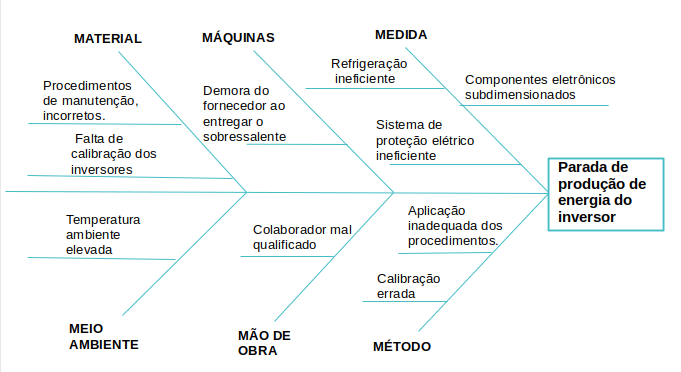
\includegraphics[width=1\textwidth]{images/ishikawa_aplicacao.png}
    \caption*{Fonte: SunBurn.}
    \label{fig:ishikawa_aplicacao}
  \end{figure}

  
  \begin{figure}[H]
    \caption{Diagrama de Correlação} %!ALTERAR A IMAGEM POIS FALTA LEGENDA NO EIXO Y
    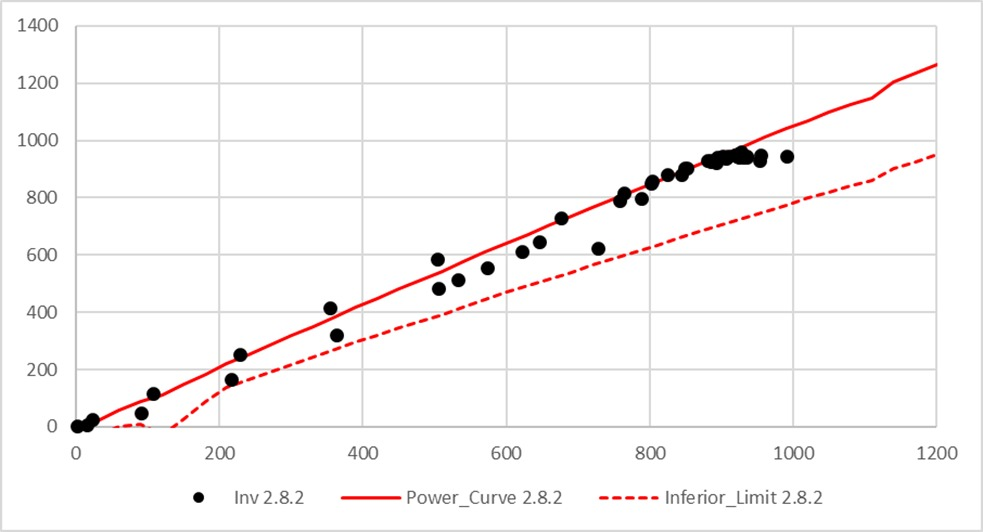
\includegraphics[width=1\textwidth]{images/correlacao_1.jpeg}
    \caption*{Fonte: SunBurn.}
    \label{fig:correlacao1_aplicacao}
  \end{figure}

  
  \begin{figure}[H]
    \caption{Diagrama de Correlação.} %!ALTERAR A IMAGEM POIS FALTA LEGENDA NO EIXO Y
    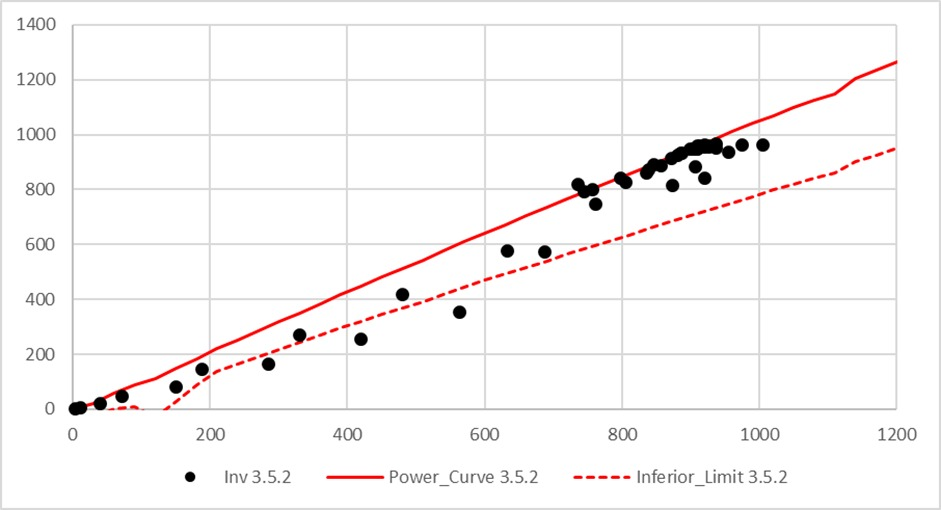
\includegraphics[width=1\textwidth]{images/correlacao_2.jpeg}
    \caption*{Fonte: SunBurn.}
    \label{fig:correlacao2_aplicacao}
  \end{figure}

  
  \begin{figure}[H]
    \caption{Checklist aplicado a Operação e Manutenção.} %!ALTERAR A IMAGEM POIS FALTA LEGENDA NO EIXO Y
    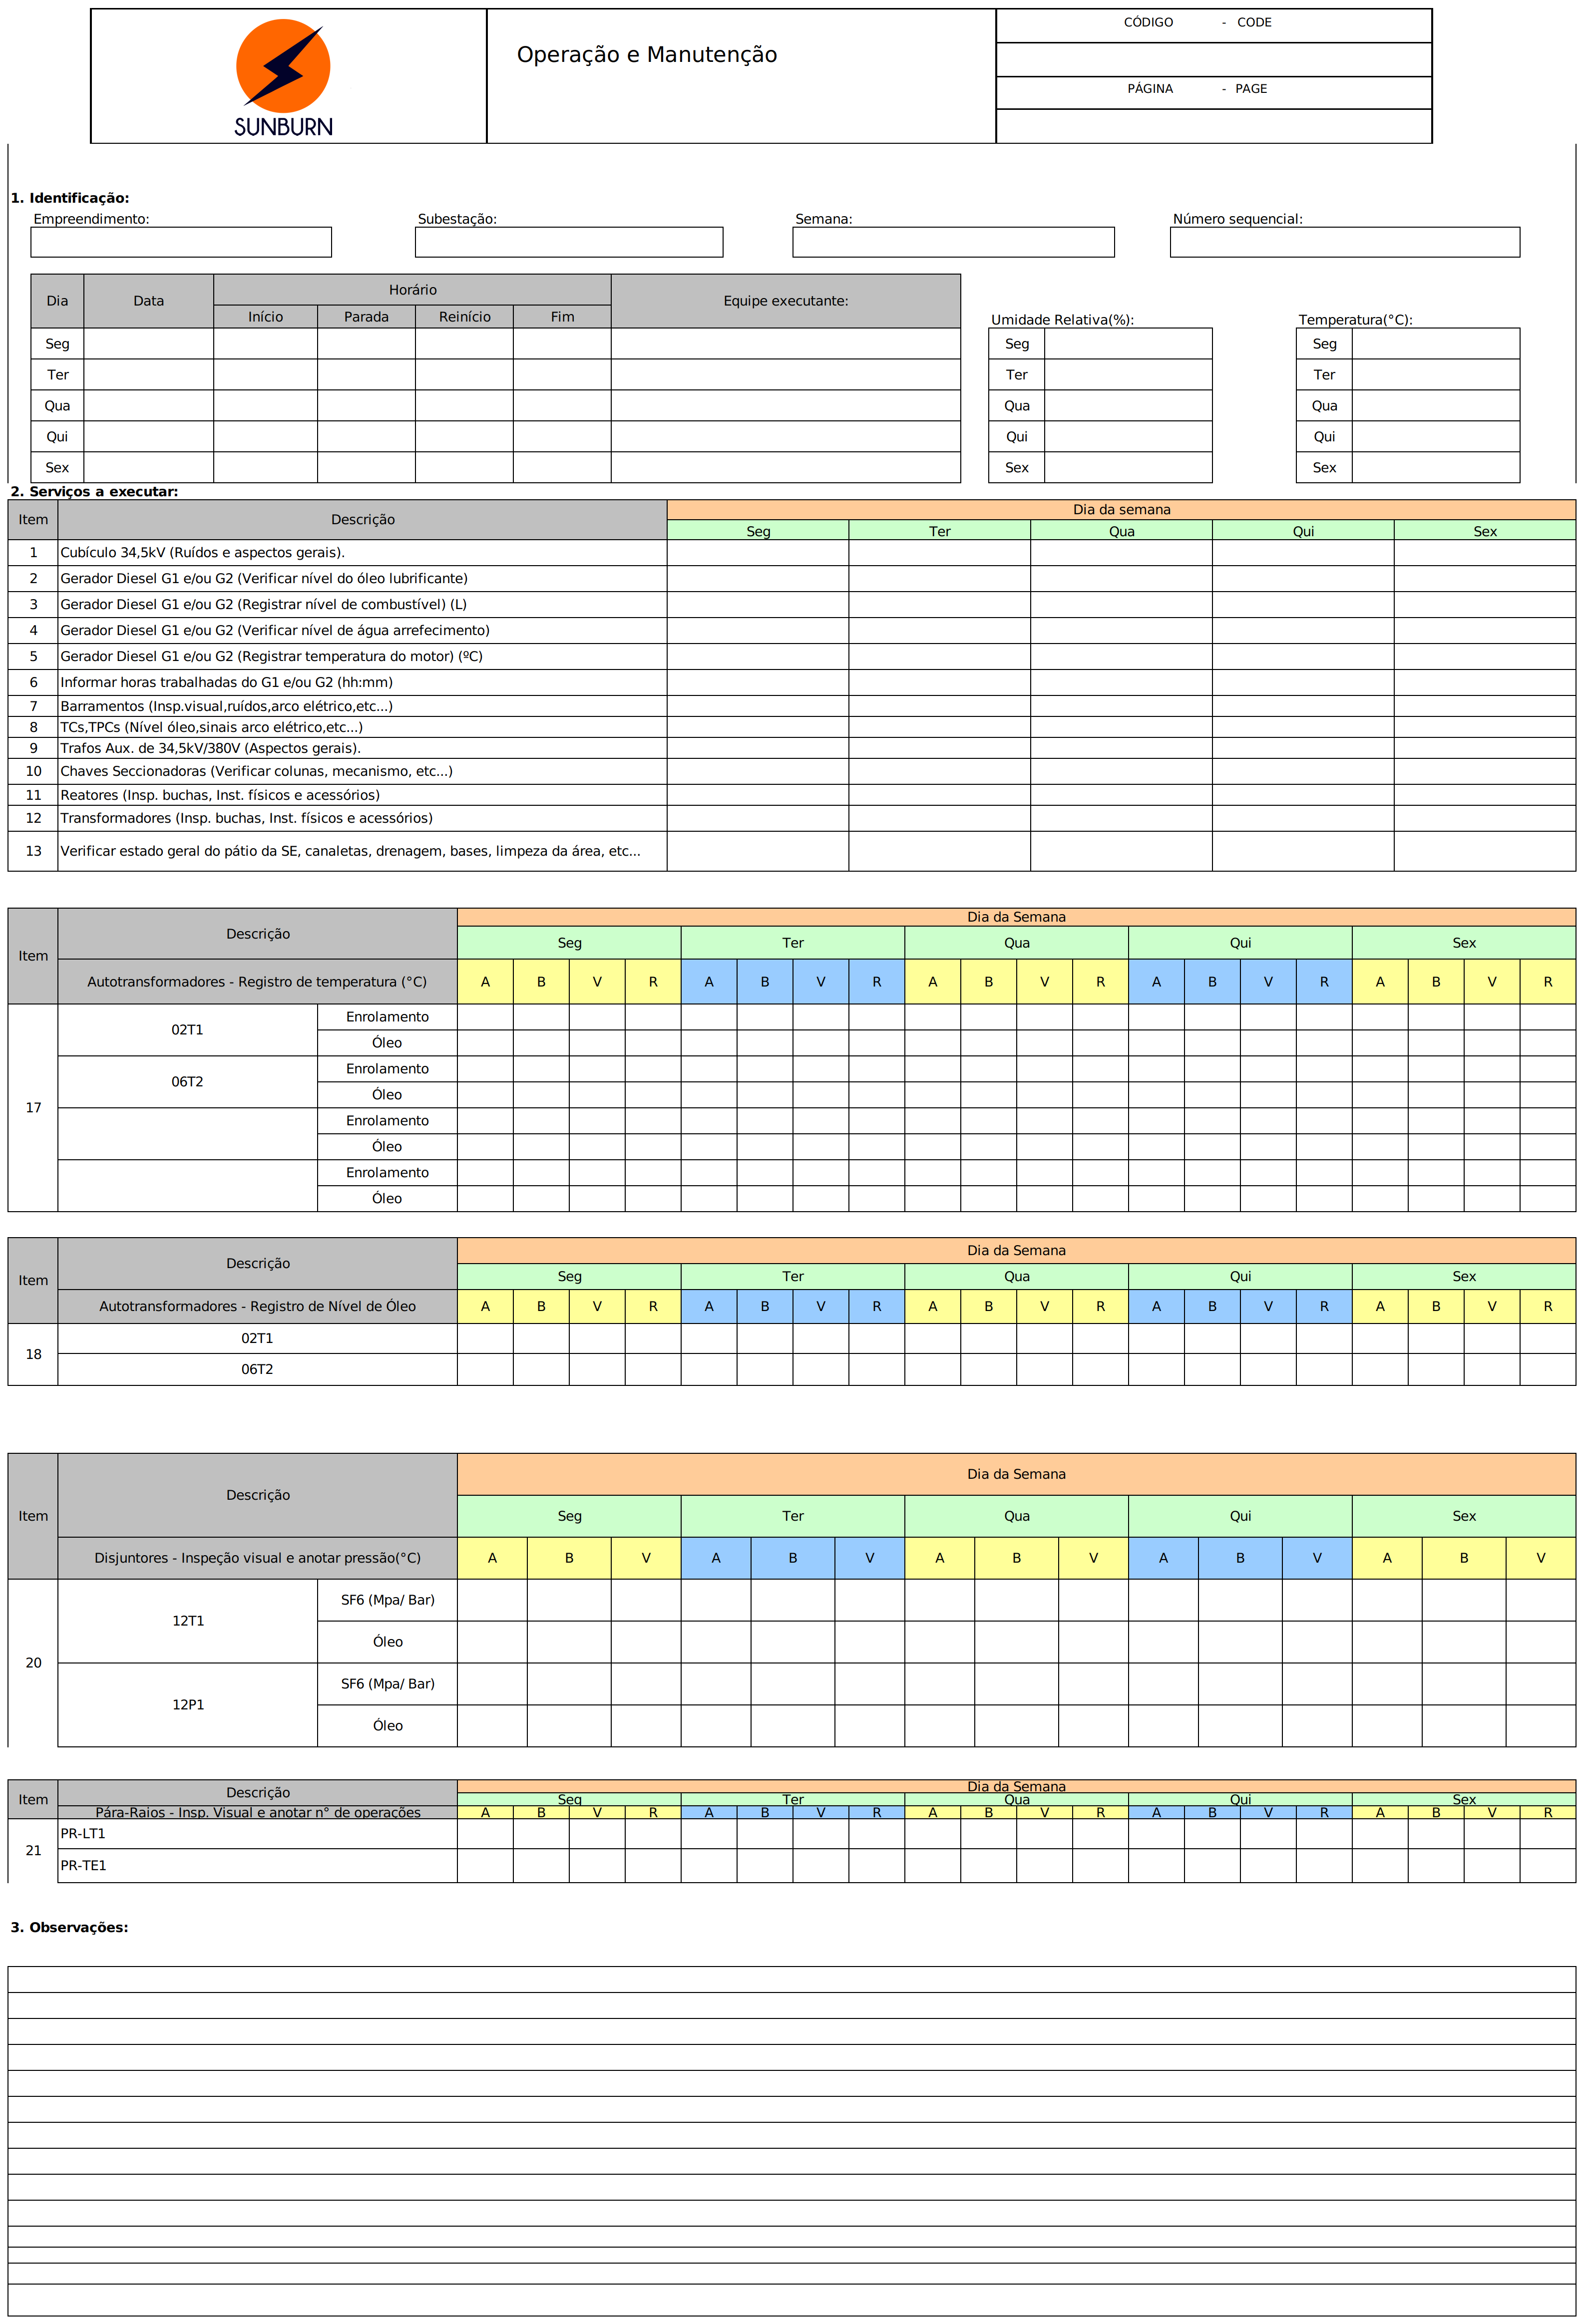
\includegraphics[width=1\textwidth]{images/checklist_aplicacao.png}
    \caption*{Fonte: SunBurn.}
    \label{fig:checklist_aplicacao}
  \end{figure}
  
	\chapter{CONFIABILIDADE E MANUTENÇÃO DO SISTEMA PRODUTIVO}
\label{chap:confiabilidade_manutencao_do_sistema_produtivo}
Sempre há a probabilidade das coisas saírem erradas, todavia, em alguns casos é vital que os produtos ou serviços não falhem. Aceitar que falhas ocorrerão não é o mesmo que ignorá-las. É importante estudar ``como'' e ``por que'' as coisas falham para que possamos minimizar o surgimento destes erros.

A Confiabilidade é uma importante forma de estudar as falhas e mede a probabilidade de uma falha não ocorrer. Outras maneiras, como a taxa de falhas, que mede a frequência de acontecimento da falha e a disponibilidade, que é o período de tempo útil disponível para a operação também são usados frequentemente. A observação e ação em cima destes pontos fazem com que as atividades da operação reduzam drasticamente os seus pontos de falha.

Outro ponto a ser observado para manter a qualidade do processo é a manutenção. A mesma oferece uma lista de benefícios que contribuem diretamente com o aumento da confiabilidade dos produtos e da produção. Dividida principalmente em 3 modelos, a manutenção pode ser corretiva, a ação após o acontecimento da falha; preventiva, ação pré-acontecimento ou preditiva, ações de monitoramento visando a previsão de erros. Estas três estratégias podem ser usadas individualmente ou também combinadas entre sí.

%--------------------------------------------------------------
\section{Sec1}
\label{sec:confiabilidade_manutencao_sec1}




%------------------------------------------------------------------
\section{Aplicação Prática}
\label{sec:confiabilidade_manutencao_aplicacao}

	\chapter{CONCLUSÃO}
\label{chap:conclusao}

Este trabalho apresentou um estudo das aplicações dos diversos conceitos relacionados aos Sistemas Produtivos (Industriais) na empresa SunBurn. A empresa SunBurn, nome fictício, é uma empresa geradora de energia elétrica localizada no nordeste do Brasil, em função dos elevados níveis de insolação, e que tem a concessionária de distribuição regional como seu único cliente. O processo produtivo desta empresa é caracterizado pela conversão de energia solar em energia elétrica através do modelo de produção contínuo com demanda dependente.

A empresa emprega técnicas de \ac{MRP} providas pela \ac{SAP} para o seu controle de estoques de materiais utilizados na manutenção do processo produtivo. Além disso, apesar do processo de produção ser do tipo contínuo e diretamente entregue ao sistema de transporte, linhas de transmissão, com controle de geração baseado na demanda prevista com base em modelos e dados históricos, a produção da SunBurn não segue o modelo \textit{Just In Time}. Assim, a cadeia de suprimentos da mesma é centrada, à montante, no suprimento de equipamentos e materiais necessários para a manutenção da unidade produtiva e, à jusante, na venda do produto exclusivamente para o distribuidor regional.

Pode-se inferir através do processo de conversão de energia apresentado neste trabalho, que a correta manutenção (preventiva, preditiva e corretiva) dos equipamentos e estruturas do parque industrial influenciam fortemente na capacidade produtiva desta empresa. A falha de poucos equipamentos pode ocasionar uma paralisação de uma parte considerável do processo produtivo, ou até mesmo, sua completa estagnação. A Por isso, a empresa apresenta um conjunto de processos relacionados ao controle do seu processo industrial e na manutenção do mesmo com o emprego das técnicas como Diagramas de Ishikawa, Diagramas de Correlação e \textit{Checklists}, dentre outras.

Finalmente, através das análises realizadas, acredita-se que o trabalho aqui apresentado consegue correlacionar os conteúdos estudos durante a disciplina de Sistemas Produtivos ministrada pelo Prof. Dr. Francisco Uchoa Passos durante o segundo semestre de 2020 junto ao SENAI CIMATEC com as práticas utilizadas por uma empresa existente e atuante no mercado brasileiro, ressalvados os dados e ou procedimentos que foram caracterizados como confidenciais pela empresa em questão.

% --------------------------------------------------------------------------
% Referências
	% \cleardoublepage
	\titleformat{\chapter}[display]{\vspace*{-24pt}\ABNTEXchapterfont\large\bfseries}{\chaptertitlename\ \thechapter}{12pt}{\Large}
	\bibliography{bibliography}
% --------------------------------------------------------------------------
% Apêndices
	% \apendices
	% \justify
	% %
	% \chapter{Questões de abordagem à pesquisa}
	% \label{apend:quest}
	% %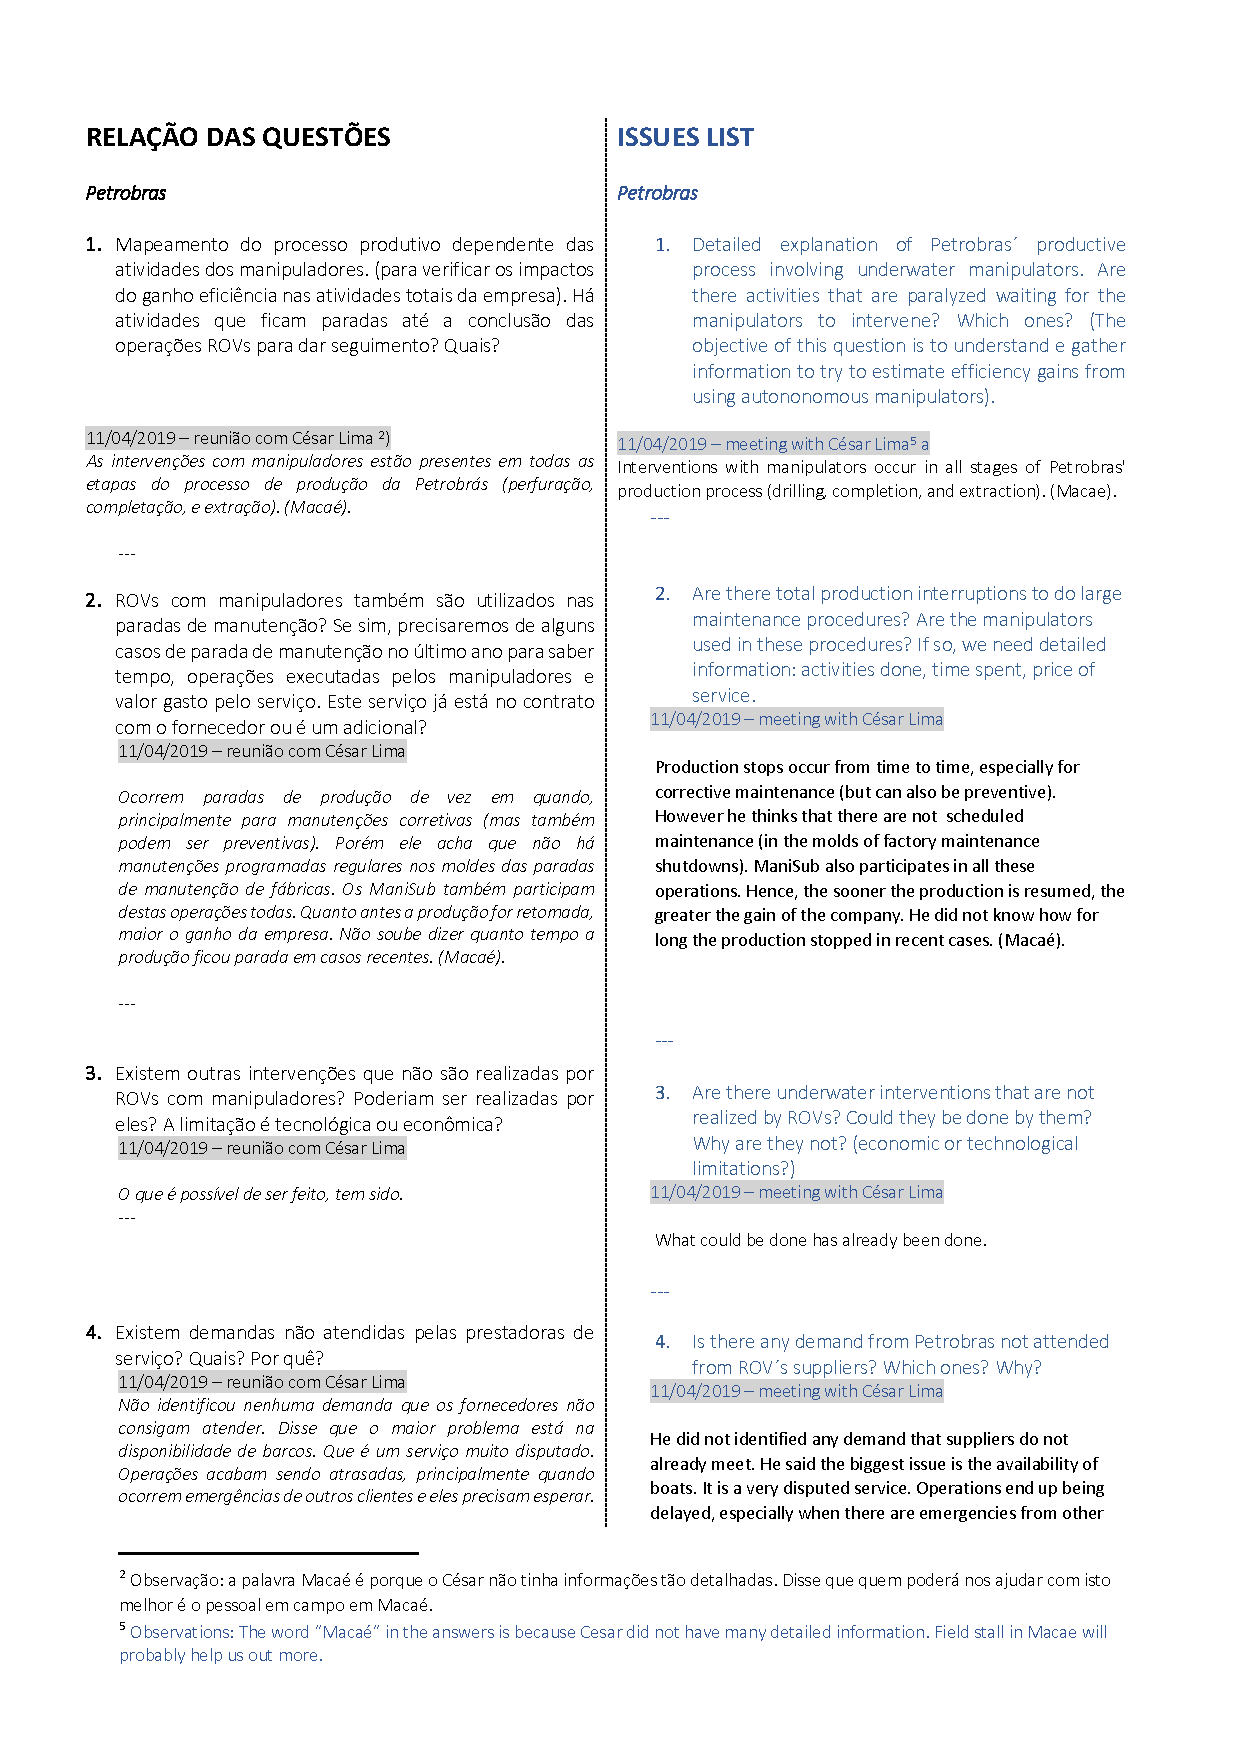
\includepdf[pages={{},-}]{appendix/listquest.pdf}
	% \lipsum[1] % Comentar e adicionar apêndice aqui
	% %
	% \chapter{Um assunto importante}
	% \label{apend:assunto}
	% \lipsum[1] % Comentar e adicionar apêndice aqui


% --------------------------------------------------------------------------
% % Anexos
% 	\anexos
% 	\justify
% 	%
% 	\chapter{Outro assunto importante}
% 	\label{ann:relant}
% 	%\includepdf[pages={{},-}]{annex/manisubanterioridade.pdf}
% 	\lipsum[1] % Comentar e adicionar apêndice aqui
% 	%
\end{document}